\subsection{Worksheet - Review of Damped \& Driven Harmonic Oscillators}
\begin{p}
An undamped harmonic oscillator has general solution $x(t) = B_1\cos(\omega t) + B_2\sin(\omega t)$. Show this can be recast as $x(t) = A\cos(\omega t - \delta)$, where $A = \sqrt{A^2 + B^2}$.
\end{p}
\begin{s}
Consider a right-angle triangle with side lengths $B_1$, $B_2$ and hypotenuse $A + \sqrt{B_1^2 + B_2^2}$. Then, let $\cos\delta = \frac{B_1}{A}$ and $\sin\delta = \frac{B_2}{A}$. Looking at the equation for $x(t)$ above, we can multiply it by one in a clever way:
\[x(t) = A\left[\frac{B_1}{A}\cos\omega t + \frac{B_2}{A}\sin\omega t\right] = A\left[\cos\delta\cos\omega t + \sin\delta \sin\omega t\right] = A\cos(\omega t - \delta)\]
Where the last equality follows by a trigonometric identity.
\end{s}

\begin{p}
Show that the kinetic and potential energy of a simple undamped oscillator have the same amplitude but are out of phase, such that the total energy is conserved. 
\end{p}
\begin{s}
Using our equation for $x(t)$ above (where $x(t)$ is the displacement from equilibrium), the total energy is given by:
\[E = U + T = \frac{1}{2}kx^2 + \frac{1}{2}m\dot{x}^2 = \frac{1}{2}kA^2\cos^2(\omega t - \delta) + \frac{1}{2}mA^2\omega^2\sin^2(\omega t - \delta)\]
We have that $\omega^2 = \frac{k}{m}$ so:
\[\frac{k}{2}A^2\cos^2(\omega t - \delta) + \frac{k}{2}A^2\sin^2(\omega t - \delta) = \frac{kA^2}{2}\]
And hence the total energy is a constant; we can therefore see that $\od{E}{t} = 0$ and that the total energy is conserved.
\end{s}

\begin{p}
Damped oscillatons are described by the ODE $\ddot{x} + 2\beta\dot{x} + \omega_0^2x = 0$. Show that for overdamped motion, the decay "constant" (decay parameter) for a damped oscillator decreases with increasing friction. Sketch the decay parameters vs. $\beta$ for the whole range of $\beta$.
\end{p}
\begin{s}
We guess a solution of the form $x(t) = \exp(rt)$. We can therefore generate a characteristic equation for $r$, by substituting in the solution into the ODE and then cancelling out the exponential terms (as these can never be zero). Hence, we have:
\[r^2 + 2\beta r  + \omega_0^2 = 0\]
This is a quadratic equation with solutions:
\[r = -\beta \pm \sqrt{\beta^2 - \omega_0^2}\]
There are now different possibilities for the damping depending on the ratio of $\beta$ and $\omega_0$. For $\beta > \omega_0$, the oscillator is overdamped. For $\beta < \omega_0$, the oscillator is underdamped. For $\beta = \omega_0$, the oscillator is critically damped. Let us now consider the overdamped case. Then, we have that the discriminant in the equation above $\beta^2 - \omega_0^2$ is positive, and the general solution is the sum of decaying exponentials:
\[x(t) = C_1\exp(r_1 t) + C_2\exp(r_2 t) \]
where $r_1 = -\beta + \sqrt{\beta^2 - \omega^2}, r_2 = -\beta - \sqrt{\beta^2 - \omega^2}$. The dominant term will be the $\exp(r_1 t)$ term as this decays more slowly. Therefore, the decay parameter is:
\[-\beta + \sqrt{\beta^2 -\omega_0^2}\]
Which decreases with increasing $\beta$. We will also have a decay parameter for the underdamped case. In this case, the decay parameter is just $\beta$, as the discriminant is negative, and hence the solution $x(t)$ is composed of an oscillating part (the imaginary exponential part from the square root) and a real exponentially decaying part ($\exp(-\beta t)$). Hence the decay parameter increases linearly in this regime. Overall, we obtain a plot that looks like the follows:

Where the decay parameter is maximized when $\beta = \omega_0$, where we have critical damping.
\begin{center}
    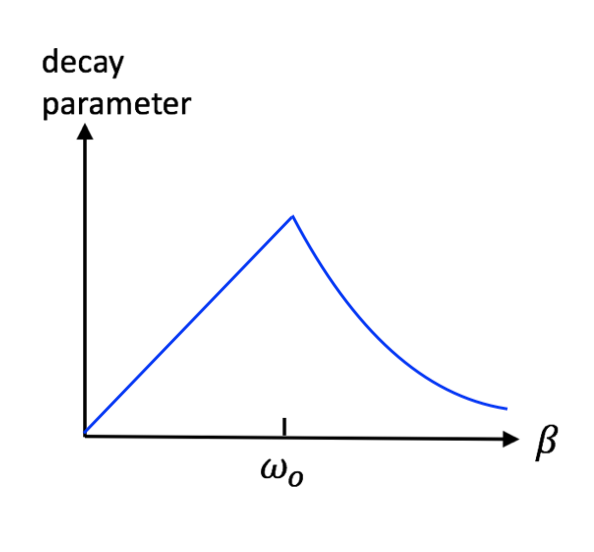
\includegraphics[scale=0.5]{Lecture-9/w9-img1.png}
\end{center}
\end{s}

\begin{p}
Show that for critical damping, the solution $x(t) = te^{rt}$ solves the ODE $\ddot{x} + 2\beta\dot{x} + \omega_0^2x = 0$. Find $r$. Write the general solution.
\end{p}
\begin{s}
For critical damping, we have that $\beta = \omega_0$ and we can calculate $r$ to be:
\[r = -\beta \pm \sqrt{\beta^2 - \beta^2} = -\beta\]
Hence one solution is given by:
\[x_1(t) = C_1\exp(-\beta t)\]
And we check the Ansatz provided in the question to verify it as a second solution. The first time derivative is given by:
\[\dot{x} = \exp(rt) + rt\exp(rt)\]
And the second time derivative as:
\[\ddot{x} = r\exp(rt) + r\exp(rt) + r^2t\exp(rt) = 2r\exp(rt) + r^2t\exp(rt)\]
So substituting this into the ODE, with $r = -\beta$:
\[-2\beta\exp(-\beta t) + \beta^2t\exp(-\beta t) + 2\beta\left(\exp(-\beta t) - \beta t\exp(-\beta t)\right) + \beta^2t\exp(-\beta t) = 0\]
So we can see that this is indeed a solution! Hence the general solution is given by:
\[x(t) = C_1\exp(-\beta t) + C_2 t\exp(-\beta t)\]
\end{s}

\begin{p}
Find the condition on $C$ for $z(t) = Ce^{i\omega t}$ to be a solution to $\ddot{z} + 2\beta\dot{z} + \omega_0^2z = f_0e^{i\omega t}$. Express the coefficient $C$ as $Ae^{-i\delta}$ and find $A$ and $\delta$.
\end{p}
\begin{s}
Let us plug in $z(t)$ into the ODE:
\[(-\omega^2 + 2i\beta\omega + \omega_0^2)C\exp(i\omega t) = f_0\exp(i\omega t)\]
We may cancel out the exponentials on both sides:
\[(-\omega^2 + 2i\beta\omega + \omega_0^2) =f_0\]
Hence we find:
\[C = \frac{f_0}{-\omega^2 + 2i\beta\omega + \omega_0^2} = A\exp(i\delta)\]
We have that $A^2 = CC^*$ and so:
\[A^2 = \frac{f_0}{-\omega^2 + 2i\beta\omega + \omega_0^2}\frac{f_0}{-\omega^2 - 2i\beta\omega + \omega_0^2} = \frac{f_0^2}{(\omega_0^2 - \omega^2)^2 + 4\beta^2\omega^2}\]
To get the phase, we see that:
\[f_0\exp(i\delta) = A(\omega_0^2 - \omega^2 + 2i\beta\omega)\]
And solving (using some knowledge of complex numbers and extracting their phase) we get:
\[\delta = \arctan(\frac{\Im}{\Re}) = \arctan(\frac{2\beta \omega}{\omega_0^2 - \omega^2})\]
\end{s}

\begin{p}
Write the general solution to $\ddot{x} + 2\beta\dot{x} + \omega_0^2x = f_0\cos(\omega t)$ for the underdamped case. What are the two undetermined constants?
\end{p}
\begin{s}
Writing the general solution, we have:
\[x(t) = A\cos(\omega t -\delta) + C_1\exp(r_1 t) + C_2\exp(r_2 t)\]
Where the first term is the particular solution (comes from the driving) and the exponentials come from the homogenous solution. The former is the long-term oscillatory behavior, the latter is the transient solution (the exponentials decay away with time).
\end{s}

\begin{p}
Show that the Q-factor given by the ratio of the width to the mean of the resonance curve is equal to $\pi$ times the number of oscillations in one decay time.
\end{p}
\begin{s}
When $\omega \sim \omega_0$ (when the driving frequency approaches the natural frequency), we notice a resonance phenomenon, where the amplitude of the driven oscillator gets very large (technically it is slightly off from $\omega = \omega_0$, but to good approximation it is at the natural frequency of the system). This is pictured below:
\begin{center}
    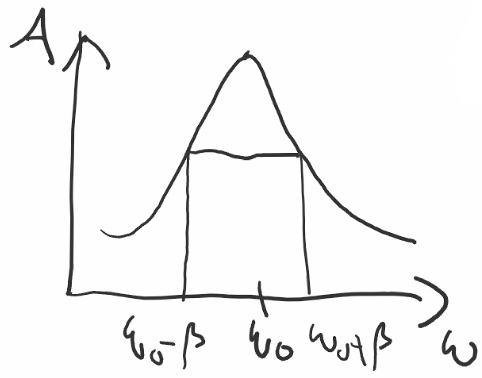
\includegraphics[scale=0.5]{Lecture-9/w9-img2.png}
\end{center}
We can also consider the width of the resonance peak. It is defined as:
\[Q = \frac{\omega_0}{2\beta}\]
Stronger damping implies a smaller quality factor and a narrower peak, and weak damping implies a larger quality factor and a broadened peak. To prove the claim provided in the question, we consider that the decay time is given by $\tau = \frac{1}{\beta}$ and the period is $T = \frac{2\pi}{\omega_0}$, so plugging this in we can immediately see that:
\[Q = \frac{\omega_0}{2\beta} = \frac{\frac{1}{\beta}\pi}{\frac{2\pi}{\omega_0}} = \pi\frac{\tau}{T}\]
which is the desired result.
\end{s}

\begin{p}
Find the phase shift at resonance when the driving frequency $\omega$ is varied. Sketch the phase shift $\delta$ vs. $\omega$.
\end{p}
\begin{s}
The phase shift is given by $\delta = \frac{\pi}{2}$ (perfectly out of phase). We can see this as the phase shift is given above by:
\[\delta = \arctan(\frac{2\beta\omega}{\omega_0^2 - \omega^2})\]
And at resonance we have $\omega \sim \omega_0$, so therefore the argument fo the arctan goes to infinity, and hence the value of $\delta$ goes to $\frac{\pi}{2}$.
\end{s}